\documentclass[journal,a4paper,twoside]{sty/IEEEtran}

%% Based on bare_jrnl.tex V1.3 2007/01/11 by Michael Shell (requires IEEEtran.cls version 1.7 or later) 

\usepackage[utf8]{inputenc}
\usepackage[slovene]{babel}
\usepackage{sty/EVrevija}

% *** GRAPHICS RELATED PACKAGES ***
\ifCLASSINFOpdf
\usepackage[pdftex]{graphicx}
\usepackage{amsfonts}           %doda zbirko matematičnih znakov
\usepackage{graphicx}           %prikz slik  
\usepackage{longtable}          %paket za tabele, ki se raztezajo čez več strani
\usepackage{float}
\usepackage{caption}
\usepackage{color}
\usepackage{mathtools}
\usepackage{amsmath}
\usepackage{media9}
\usepackage{enumerate}
\usepackage[official]{eurosym}
\usepackage{algorithm}
\usepackage[noend]{algpseudocode}
\else % or other class option (dvipsone, dvipdf, if not using dvips).
   \usepackage[dvips]{graphicx}
\fi
%\usepackage{epsfig}
\usepackage{epstopdf} % A.T. include eps images in pdftex (Miktex2.8 or higher)

% Include all other packages here
\usepackage{textcomp} % need for \textmu
%\usepackage{eurosym} %  symbol \euro
%\usepackage[cmex10]{amsmath} % *** MATH PACKAGES ***

% correct bad hyphenation here
%\hyphenation{op-tical net-works semi-conduc-tor}

\begin{document}

% naslov prispevka, lahko uporabite en linebreak \\
\title{Rekonstrukcija objekta in poravnava oblakov točk}

\authors{Martin Knap$^1$, Janez Lapajne$^1$} % use ^1, ^2 for author(s) from different institutions

\address{Univerza v Ljubljani, Fakulteta za elektrotehniko, Tržaška 25, 1000 Ljubljana, Slovenija\\
E-pošta: janez.lapajne@gmail.com, knap.martin@gmail.com}

\abstract{V nalogi je obravnavan postopek 3D rekonstukcije objektov na podlagi več zajetih slik. Za rekonstrukcijo je uporabljena FBP (angl. \textit{Filtered Backprojection }) metoda. Temelji na rekonstrukciji 3D oblike iz slik, ki so zajete pri znanih kotih zasuka objekta. Velik poudarek je namenjen izgradnji in zasnovi sistema, saj je od njegove postavitve odvisna kakovost zajetih slik.  Osredotočamo se predvsem na elemente, ki nam pomagajo pri čimboljši rekonstrukciji objekta v obliki oblaka točk. Prikazana je kalibracija sistema in preslikava slik v metrični koordinatni sistem. Predstavljena je uporabnost rekontrukcije objektov in izvedba vzvratnega inženirstva skeniranega objekta.
}

\keywords{rekonstrukcija 3D objekta, kalibracija kamere, poravnava oblakov točk, vzvratno inženirstvo}



% Priimki avtorjev in kratek naslov članka za tekočo glavo
\markboth{M. Knap, J. Lapajne}{Rekonstrukcija objekta in poravnava oblakov točk}

% make the title area
\maketitle


\section{Uvod}
V robotskem vidu in računalniški grafiki je 3D rekonstrukcija proces zajemanja oblike in videza realnega objekta. Proces je lahko dosežen z aktivnimi ali pasivnimi metodami. V nalogi je uporabljena pasivna FBP metoda. Uporaba rekonstrukcije lahko določi profil 3D objekta oziroma koordinate katerikoli točke na tem profilu. Digitalna slika je v našem primeru vir informacij. Za dobro rekonstrukcijo je potrebno upoštevati vizualno dispariteto, osvetlitev, performance kamere in značilnosti scene. Uporabljeno kamero je potrebno ustrezno skalibrirati in merjene točke pretvoriti v metrični koordinatni sistem. Bolje kot je zastavljen zajem slik, ustreznejši so končni rezultati. Dobro zajete slike olajšajo obdelavo. Rekonstrukcija objektov je uporabljena v različnih področjih raziskovanja. Med drugim v medicini, robotiki, računalniških igrah in v vzvratnem inženirstvu. 

\section{Teoretično ozadje}

\subsection{Kalibracija}

Pred začetkom izvedbe rekonstrukcije je potrebna geometrijska kalibracija sistema. Namen kalibracije je pridobitev parametrov toge preslikave, ki jih bomo potrebovali kasneje v algoritmu 3D rekonstrukcije s filtrirano povratno projekcijo. Cilj je projekcija iz slikovnega v metrični koordinatni sistem. Referenčne točke kalibracijskega objekta (3D) najprej togo premaknemo na mesto rotirajoče mize. Nato sledi DLT (angl. \textit{Direct Linear Transformation}) kalibracija med 3D točkami referenčnega kalibra $T_{ref},_i = (X_i, Y_i, Z_i)$ ter 2D naborom točk kalibra iz slikovnega koordinatnega sistema $t_{slik},_i = (x_i, y_i)$. Pri tem je število točk kalibracijskega objekta $i = 8$. Pri DLT kalibraciji z razcepom na singularne vrednosti rešujemo sledeči sistem:


%\begin{equation}
%\setcounter{MaxMatrixCols}{12}
%a = 
%\begin{bsmallmatrix}
%X_1 & Y_1 & Z_1 & 0 & 0 & 0 & -x_1 X_1 & -x_1 Y_1 & -x_1 Z_1 & 1 & 0 & -x_1 \\ 
%0 & 0 & 0 & X_1 & Y_1 & Z_1 & -y_1 X_1 & -y_1 Y_1 & -y_1 Z_1 & 0 & 1 & -y_1 \\
% &  &  &  &  &  & \vdots &  &  &  &  &  \\
%X_8 & Y_8 & Z_8 & 0 & 0 & 0 & -x_8 X_8 & -x_8 Y_8 & -x_8 Z_8 & 1 & 0 & -x_8 \\ 
%0 & 0 & 0 & X_8 & Y_8 & Z_8 & -y_8 X_8 & -y_8 Y_8 & -y_8 Z_8 & 0 & 1 & -y_8 \\
%\end{bsmallmatrix}
%\end{equation}

\begin{equation}
\setcounter{MaxMatrixCols}{12}
a = 
\begin{bsmallmatrix}
X_i & Y_i & Z_i & 0 & 0 & 0 & -x_i X_i & -x_i Y_i & -x_i Z_i & 1 & 0 & -x_i \\ 
0 & 0 & 0 & X_i & Y_ i& Z_i & -y_i X_i & -y_i Y_i & -y_i Z_i & 0 & 1 & -y_i \\
\end{bsmallmatrix}
\end{equation}

\begin{equation}
\setcounter{MaxMatrixCols}{12}
\textbf{p} =
\begin{bsmallmatrix}
r_{11} & r_{12} & r_{13} & r_{21} & r_{22} & r_{23} & r_{31} & r_{23} & r_{33} & t_x & t_y & t_z
\end{bsmallmatrix}
\end{equation}

\begin{equation}
a\textbf{p}^T=0
\end{equation}

Matrika $a$ ima dimenzije $16 \times 12$. Rešitev sistema predstavlja 12 parametrov toge preslikave, ki predstavljajo rotacijo $r_{ij}$ ter translacijo $t_k$.

\subsection{Filtrirana povratna projekcija}

Jedro naloge predstavlja postopek FBP (angl. \textit{Filtered Backprojection}), ki je eden od temelnjih načinov rekonstrukcije pri slikanju z računalniško tomografijo na področju zdravstva. Idejo koncepta filtrirane povratne projekcije je najenostavneje predstaviti na 2D primeru, kjer 2D merjencu $f(x,y)$ za več kotov $\theta$ zajamemo 1D prečne projekcije $p_{\theta}(r)$.

\begin{figure}[H]
	\centerline{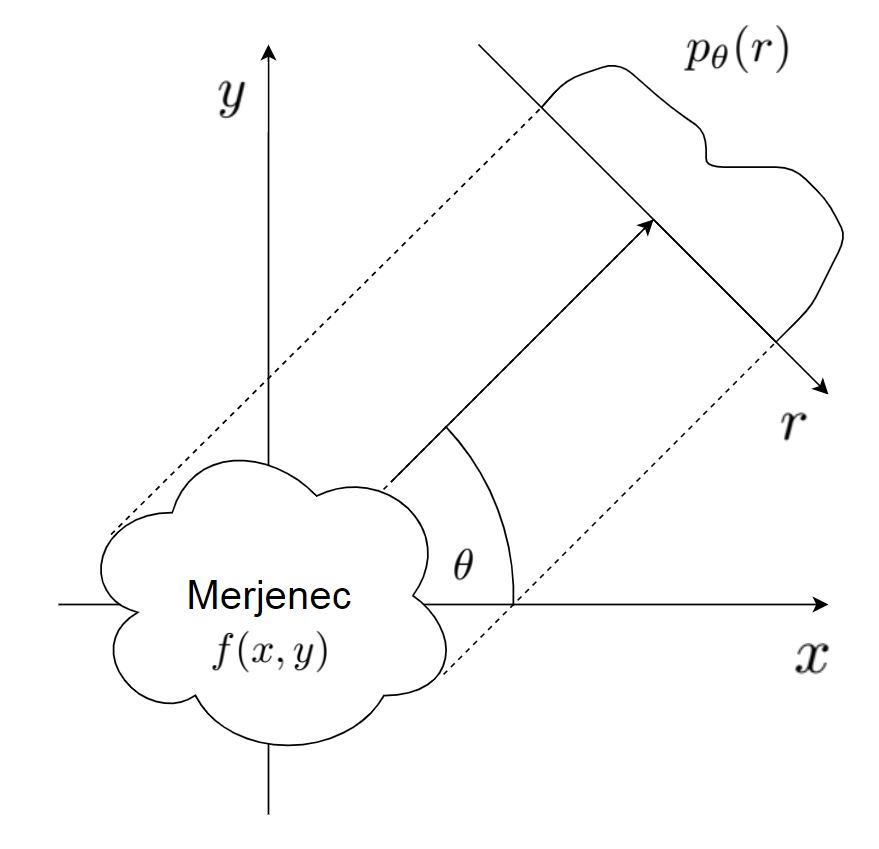
\includegraphics[width=4.5cm]{fig/FBPderi}}
	\caption{Filtrirana povratna projekcija.}
	\label{fig:fbp_deri}
\end{figure}

Zajete projekcije so nato pretvorjene v frekvenčno domeno s pomočjo Fourier-ove transformacije $P_{\theta}(\omega)$ za vsak kot. Tu nato sledi filtriranje projekcij s frekvenčnim odzivom $|\omega|$ tako, da dobimo $g_{\theta}(r) = \int  P_{\theta}(\omega)|\omega|e^{i 2\pi\omega r} d\omega$. S filtriranjem se želimo znebiti visokih frekvenc v projekcijah in posledično pridobiti kvalitetnejšo rekonstrukcijo. Po filtriranju nato sledi še rekonstrukcija v $f'(x,y)$ in sicer tako, da filtrirane inverze Fourier-ove transformacije seštejemo.

\begin{equation}
f'(x,y) = \frac{1}{2\pi} \int_{0}^{\pi} g_{\theta}(r) (x \cos\theta + y \sin \theta)d\theta
\end{equation}

Ali v diskretni obliki, kjer je $\Delta\theta$ korak diskretizacije:
\begin{equation}
f'(x,y) = \frac{1}{2\pi} \sum\limits_{i=0}^{N-1} \Delta\theta_i g_{\theta_i}(x \cos\theta_i + \sin\theta_i)
\end{equation}

Za potrebe naloge je postopek razširjen v tretjo dimenzijo, implementirani algoritem pa je predstavljen v spodnejm podpoglavju.

\subsubsection{FBP algoritem}

Na spodnji sliki je prikazan diagram poteka uporabljenjega FBP algoritma.

\begin{figure}[H]
	\centerline{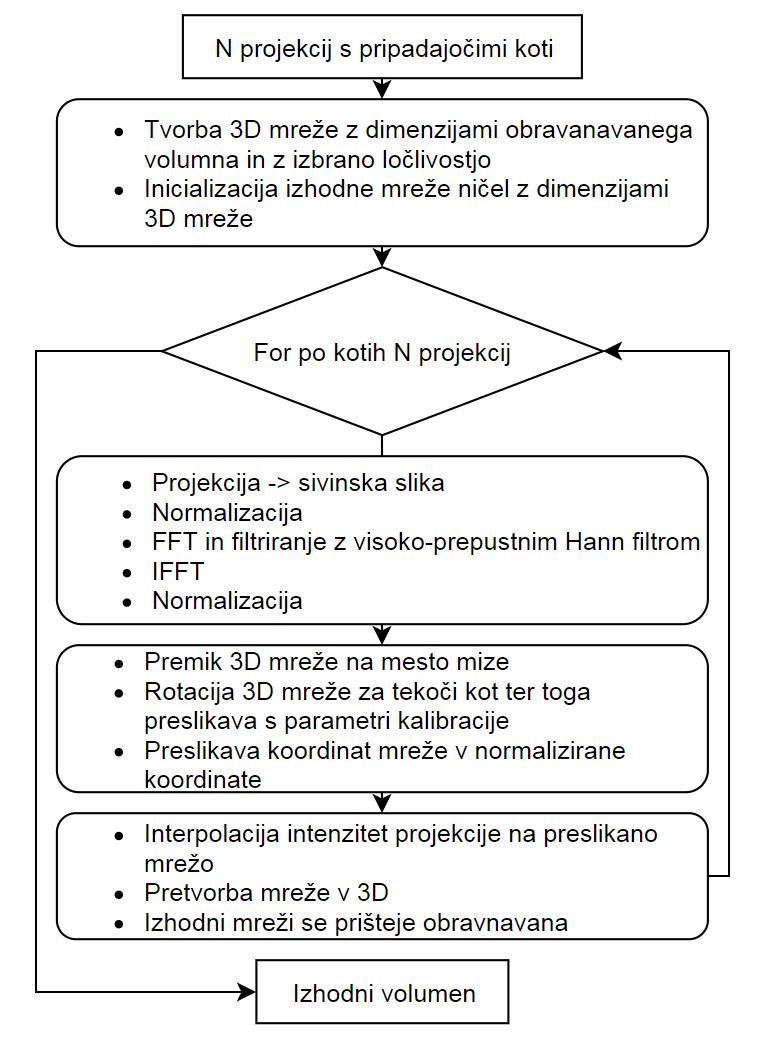
\includegraphics[width=6cm]{fig/FBPflow}}
	\caption{Diagram poteka FBP algoritma.}
	\label{fig:fbp_flow}
\end{figure}

\subsection{Poravnava oblakov točk}
%
Potek algoritma poravnave točk je prikazan na sliki ~\ref{fig:alg_poravnava}. Poravnavno izvajamo med dvema oblakoma točk tako, da enega prilagajamo na drugega. Na začetku oba oblaka točk postavimo v koordinatno izhodišče. Nato izvajamo optimizacijo prileganja na različih rotacijah prilagajočega oblaka. Slednje je izvedeno tako, da prilagajoč oblak rotiramo po 20 stopinj in v vsaki legi izvajamo optimizacijo. To ponavljamo za 360 stopinj. Na koncu med vsemi izberemo poravnano lego, ki nam zagotavlja najmanjšo povprečno napako. 

\begin{figure}[H]
	\centerline{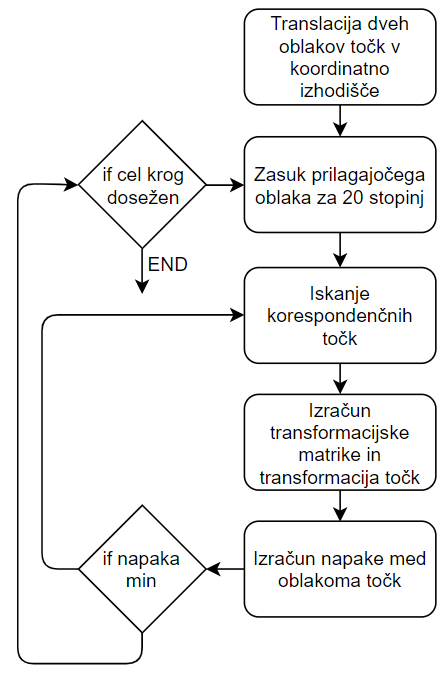
\includegraphics[width=4.5cm]{fig/alg_poravnava}}
	\caption{Potek algoritma poravnave.}
	\label{fig:alg_poravnava}
\end{figure}

\section{Zajem slik}
Sistem s katerim smo izvajali rekonstrukcijo je blokovno prikazan na sliki ~\ref{fig:blokovna}. Objekt, ki ga želimo skonstruirati postavimo na vrtljivo pozicionirno mizo. Iz zgornje strani navzdol svetimo s homogeno, difuzno osvetlitvijo. Objekta direktno ne osvetljujemo, saj je namen osvetlitve predvsem osvetlitev ozadja z enakomerno intenziteto. Cilj je doseči čimvečjo razliko v intenziteti med opazovanim objektom in zaslonom. Za ta namen je med objekt in svetilko postavljena svetlobna ovira. Slike smo zajemali z Raspberry Pi kamero v osi na objekt in na osvetljeno ozadje. Pred kamero je dodan filter za namen filtriranja okoliške svetlobe.

\begin{figure}[H]
	\centerline{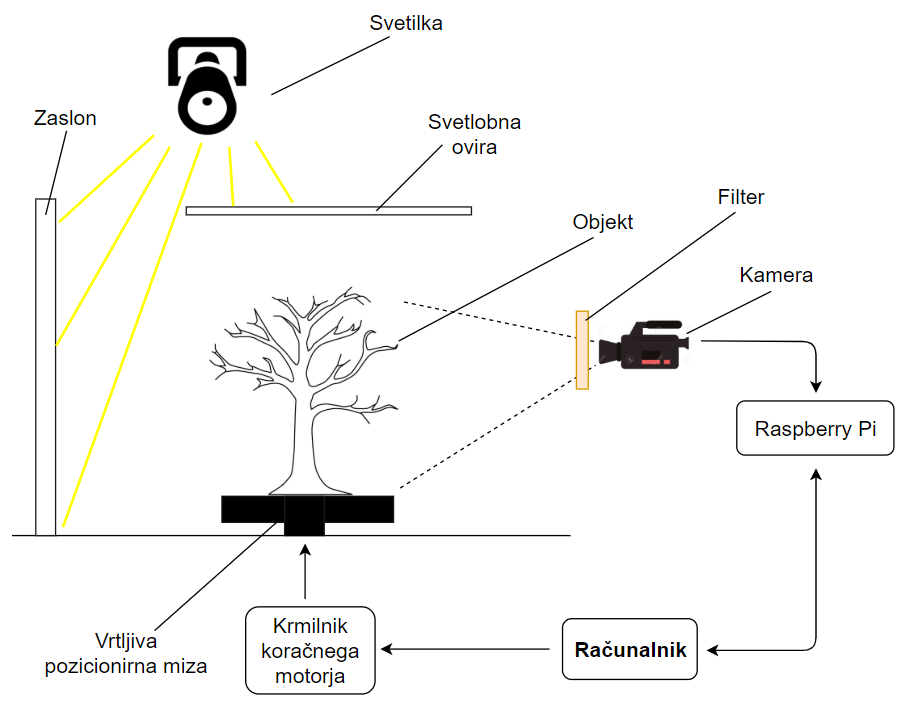
\includegraphics[width=8.2cm]{fig/blokovna_sistem}}
	\caption{Semioperacijska shema sistema.}
	\label{fig:blokovna}
\end{figure}
%
 Celoten proces zajemanja krmilnimo z računalnikom. Ta je žično povezan na krmilnik s katerim upravljamo rotirajočo pozicionirno mizo. Prav tako je računalnik brezžično povezan na Raspberry Pi. Ta zajete slike pošilja na računalnik. Objekt rekonstruiramo tako, da ga postavimo na predvideno mesto. Nato lahko pričnemo z zajemom slik. Najprej inicializiramo kamero na začetne vrednosti. Nastavimo ISO na 200, svetlost na 45 in resolucijo na 900x1000.  Objekt obračamo po začrtanih zasukih. Po vsakem izvedenem zasuku posnamemo eno sliko, ki se nato brezžično prenese iz Raspberry Pi-ja na računalnik. Postopek ponavljamo dokler objekta ne poslikamo v rangu celotnega kroga. Zajete slike ob znanih kotih zasuka se kasneje uporabijo za 3D rekonstrukcijo. V tabeli ~\ref{tab:komponente} so zapisane vse glavne komponente, ki so zajete v postavljenem sistemu. Manjše komponente kot so vijaki in nosilci v tabeli niso zajeti.

\begin{center}
	\centering
	\captionsetup{singlelinecheck = false, justification=justified}
	\captionof{table}{Komponente sistema.} 
	\label{tab:komponente} 
\begin{tabular}{|c|c|}
	\hline
	\textbf{Komponenta} & \textbf{Podrobnosti}                            \\ \hline
	Raspberry Pi        & Raspberry Pi 3 Model B                          \\ \hline
	Svetilka            & Halogenska svetilka (12V)            \\ \hline
	Zaslon              & Bela ravna plošča                               \\ \hline
	Krmilnik            & Fischertechnik stage control                \\ \hline
	Kamera              & RP Cam V2-8 MP,1080p \\ \hline
	Svetlobni filter    & Ozkopasovni filter         \\ \hline
	Svetlobna ovira     & Kartonasta zavesa                \\ \hline
		Pozicionirna miza   & Fischertechnik rotary stage                     \\ \hline
\end{tabular}
\end{center}
Primer zajete slike obravnavanega objekta z opisanim sistemom je prikazan na sliki ~\ref{fig:zajeta_slika}. S slike lahko vidimo dober kontrast objekta in precejšnjo razliko v barvi in svetlosti objekta proti ozadju. 

\begin{figure}[H]
	\centerline{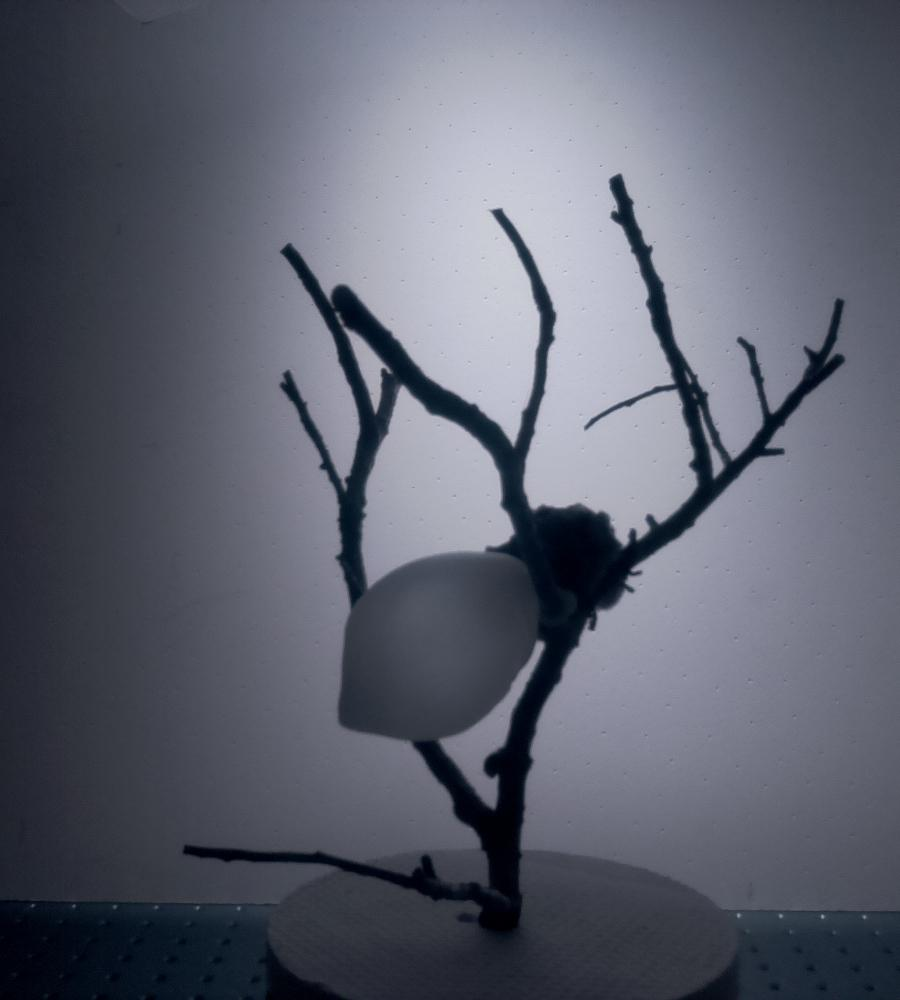
\includegraphics[width=4.2cm]{fig/zajeta_slika}}
	\caption{Zajeta slika.}
	\label{fig:zajeta_slika}
\end{figure}

\section{Rezultati}



\subsection{Vpliv kontrasta}
Testirali smo kako svetlobna pregrada vpliva na rekonstrukcijo oblaka točk. Za ta namen smo vzeli enostaven objekt s stališča rekonstrukcije. Ta je prikazan na sliki ~\ref{fig:slusalkEE}. Na levi strani je prikazana slika objekta kjer svetlobne ovire nismo uporabili. Razvidnno je, da se od objekta svetloba reflektivno odbiva v kamero. Kamera to zazna kot svetlo intenziteto. Deli objekta, ki so tako osvetljeni se po svetlosti veliko ne razlikujejo od ozadja, na nekaterih delih pa so celo zaznani, kot svetlejši. Na desni strani je prikazana slika objekta, kjer svetlobno oviro uporabimo. Objekt je v tem primeru bistveno temnejši od ozadja.

\begin{figure}[H]
	\centerline{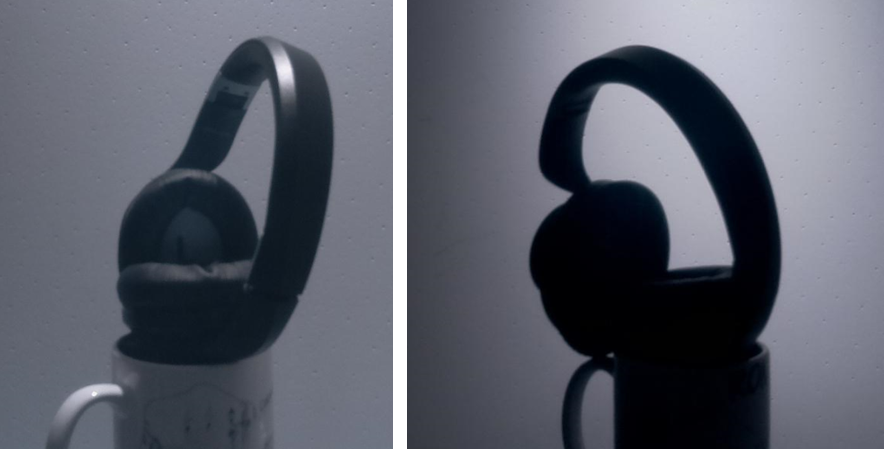
\includegraphics[width=6.2cm]{fig/slusalke_1}}
	\caption{Objekt: a) brez pregrade, b) s pregrado.}
	\label{fig:slusalkEE}
\end{figure}

Na sliki ~\ref{fig:slusalke} sta prikazana rezultata rekonstrukcij brez in z uporabo svetlobne ovire. Opazimo lahko, da je v primeru uporabljene pregrade objekt bistveno lepše rekonstruiran. V primeru, ko zavese nismo uporabili nam odboji povzročajo napačno reprezentacijo objekta. 



\begin{figure}[H]
	\centerline{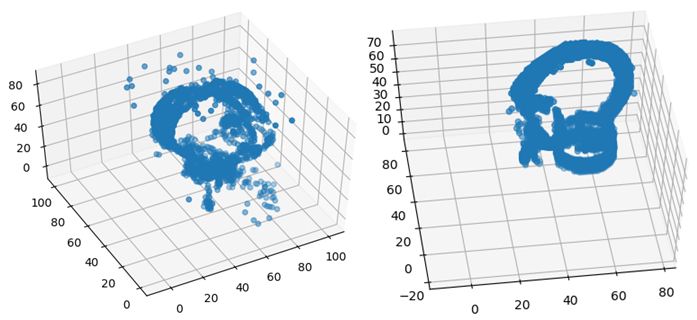
\includegraphics[width=6.2cm]{fig/slusalke}}
	\caption{Rekonstrukcija: a) brez pregrade, b) s pregrado.}
	\label{fig:slusalke}
\end{figure}


\subsection{Število zajetih slik}
Dvakrat smo rekonstruirali isti predmet. Enkrat na podlagi 30 slik in drugič na podlagi 90 slik. Opazovali smo kako število zajetih slik vpliva na rekontrukcijo. Na sliki ~\ref{fig:slika_90_30} je čisto na levi strani prikazan skeniran objekt, na sredini objekt rekonstruiran na podlagi 90 slik in na desni objekt rekonstruiran na podlagi 30 slik. Vidimo, da je dobimo boljšo obliko na podlagi večih slik. Za prikaz celotnega objekta v obeh primerih bi bilo potrebno prilagoditi meje upragovanja. 
%
\begin{figure}[H]
	\centerline{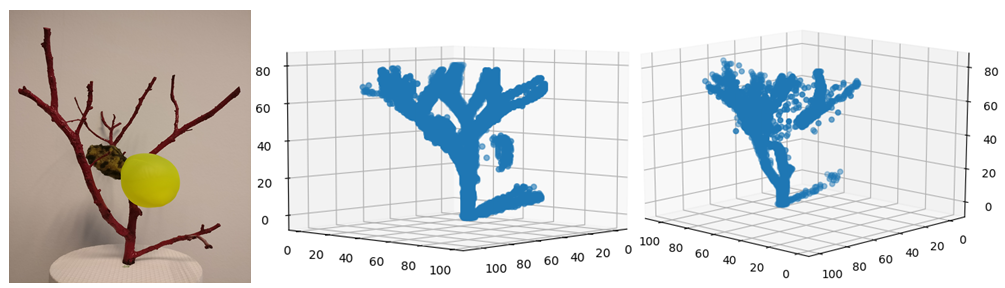
\includegraphics[width=8cm]{fig/slika_90_30}}
	\caption{a) objekt, b) zajetih 90 slik, c) zajetih 30 slik.}
	\label{fig:slika_90_30}
\end{figure}
%
%
\subsection{Poravnava oblakov točk}
Za dodaten eksperiment smo izvedli medsebojno poravnavo oblakov točk. Referenčni oblak točk smo zajeli z 90 slikami in si zapolnili referenčno lego objekta na pozicionirni mizi. Nato smo izvedli še šest zajemov po 30 slik. Ob vsakem zajemu smo skeniran objekt zasukali za predpisan kot glede na referenčno lego okoli vertikalne osi. Tako smo zajeli oblake točk zasukane za 45, 90, 135, 180, 225 in 315 stopinj. Na sliki ~\ref{fig:poravnava} sta zaradi preglednosti prikazana le referenčni oblak in oblak zasukan za 90 stopinj. Na levi strani sta oblaka prikazana pred poravnavo in na desni po poravnavi. 

\begin{figure}[H]
	\centerline{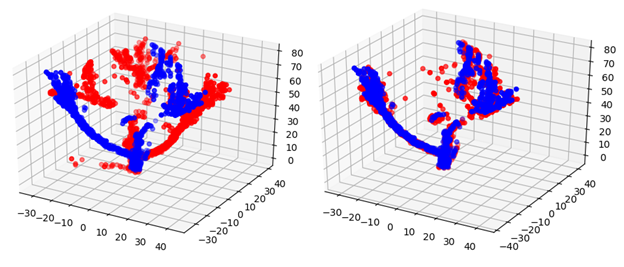
\includegraphics[width=8cm]{fig/poravnava}}
	\caption{a) neporavnana, b) poravnana.}
	\label{fig:poravnava}
\end{figure}
%
Za vse, pod različnimi koti zajete oblake točk, smo izvedli poravnavo. Nato smo iz pridobljene transformacijske matrike izluščili rotacijo okoli vertikalne osi. Ker smo poznali kote zasuka objekta glede na referenčno lego, smo jih primerjali s temi pridobljenimi iz transformacijske matrike. Na sliki ~\ref{fig:poravnava_graf} so z rdečo barvo prikazani ročno določeni zasuki, z modro pa zasuki pridobljeni iz transformacijske matrike. Vidimo, da dobimo z izračunanimi koti na podlagi transformacijske matrike dokaj zanesljive rezultate. Prileganje testiranih zasukov glede na referenčne je v rangu petih stopinj. Napaka se verjetno pojavi zaradi napak v pozicionirnem sistemu, nenatančne meritve kota glede na referenčno lego in napake v numeričnem izračunu.

\begin{figure}[H]
	\centerline{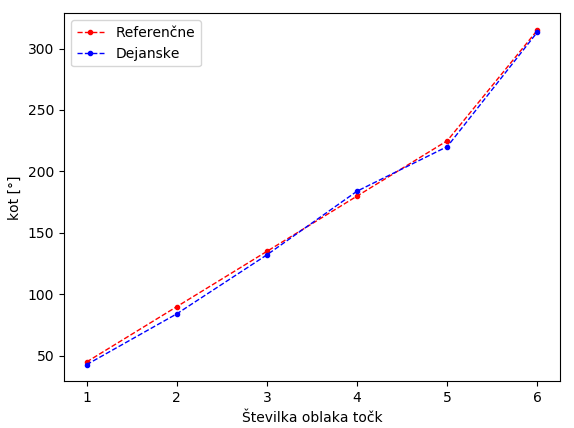
\includegraphics[width=8cm]{fig/graf_poravnave}}
	\caption{Razlika med referenčnimi in dejanskimi koti.}
	\label{fig:poravnava_graf}
\end{figure}

\subsection{Vzvratno inženirstvo}

Vzvratno inženirstvo je proces, kjer na podlagi fizičnega objekta rekonstruiramo njegov model. Model smo dobili tako, da smo z rekonstrukcijo dobljen oblak točk uvozili v 3D modelirnik Solidworks. Tam smo z uporabo posebnih orodij iz točk površine predmeta dobili površino sestavljeno iz trikotnikov in posledično zaprli vse odprtine tako, da smo dobili zaprto površino. Nato je sledila interpolacija z namenom pridobive gladkejše površine in transformacija v "trdnino". Po opravljenih korakih smo imeli model v primerni obliki za izvoz v formatu .stl. Omenjeni format se nato uvozi v razslojevalni (angl.: \textit{Slicer}), ki napravi G-kodo 3D tiskalnika za tvorbo fizičnega modela.

\begin{figure}[H]
	\centerline{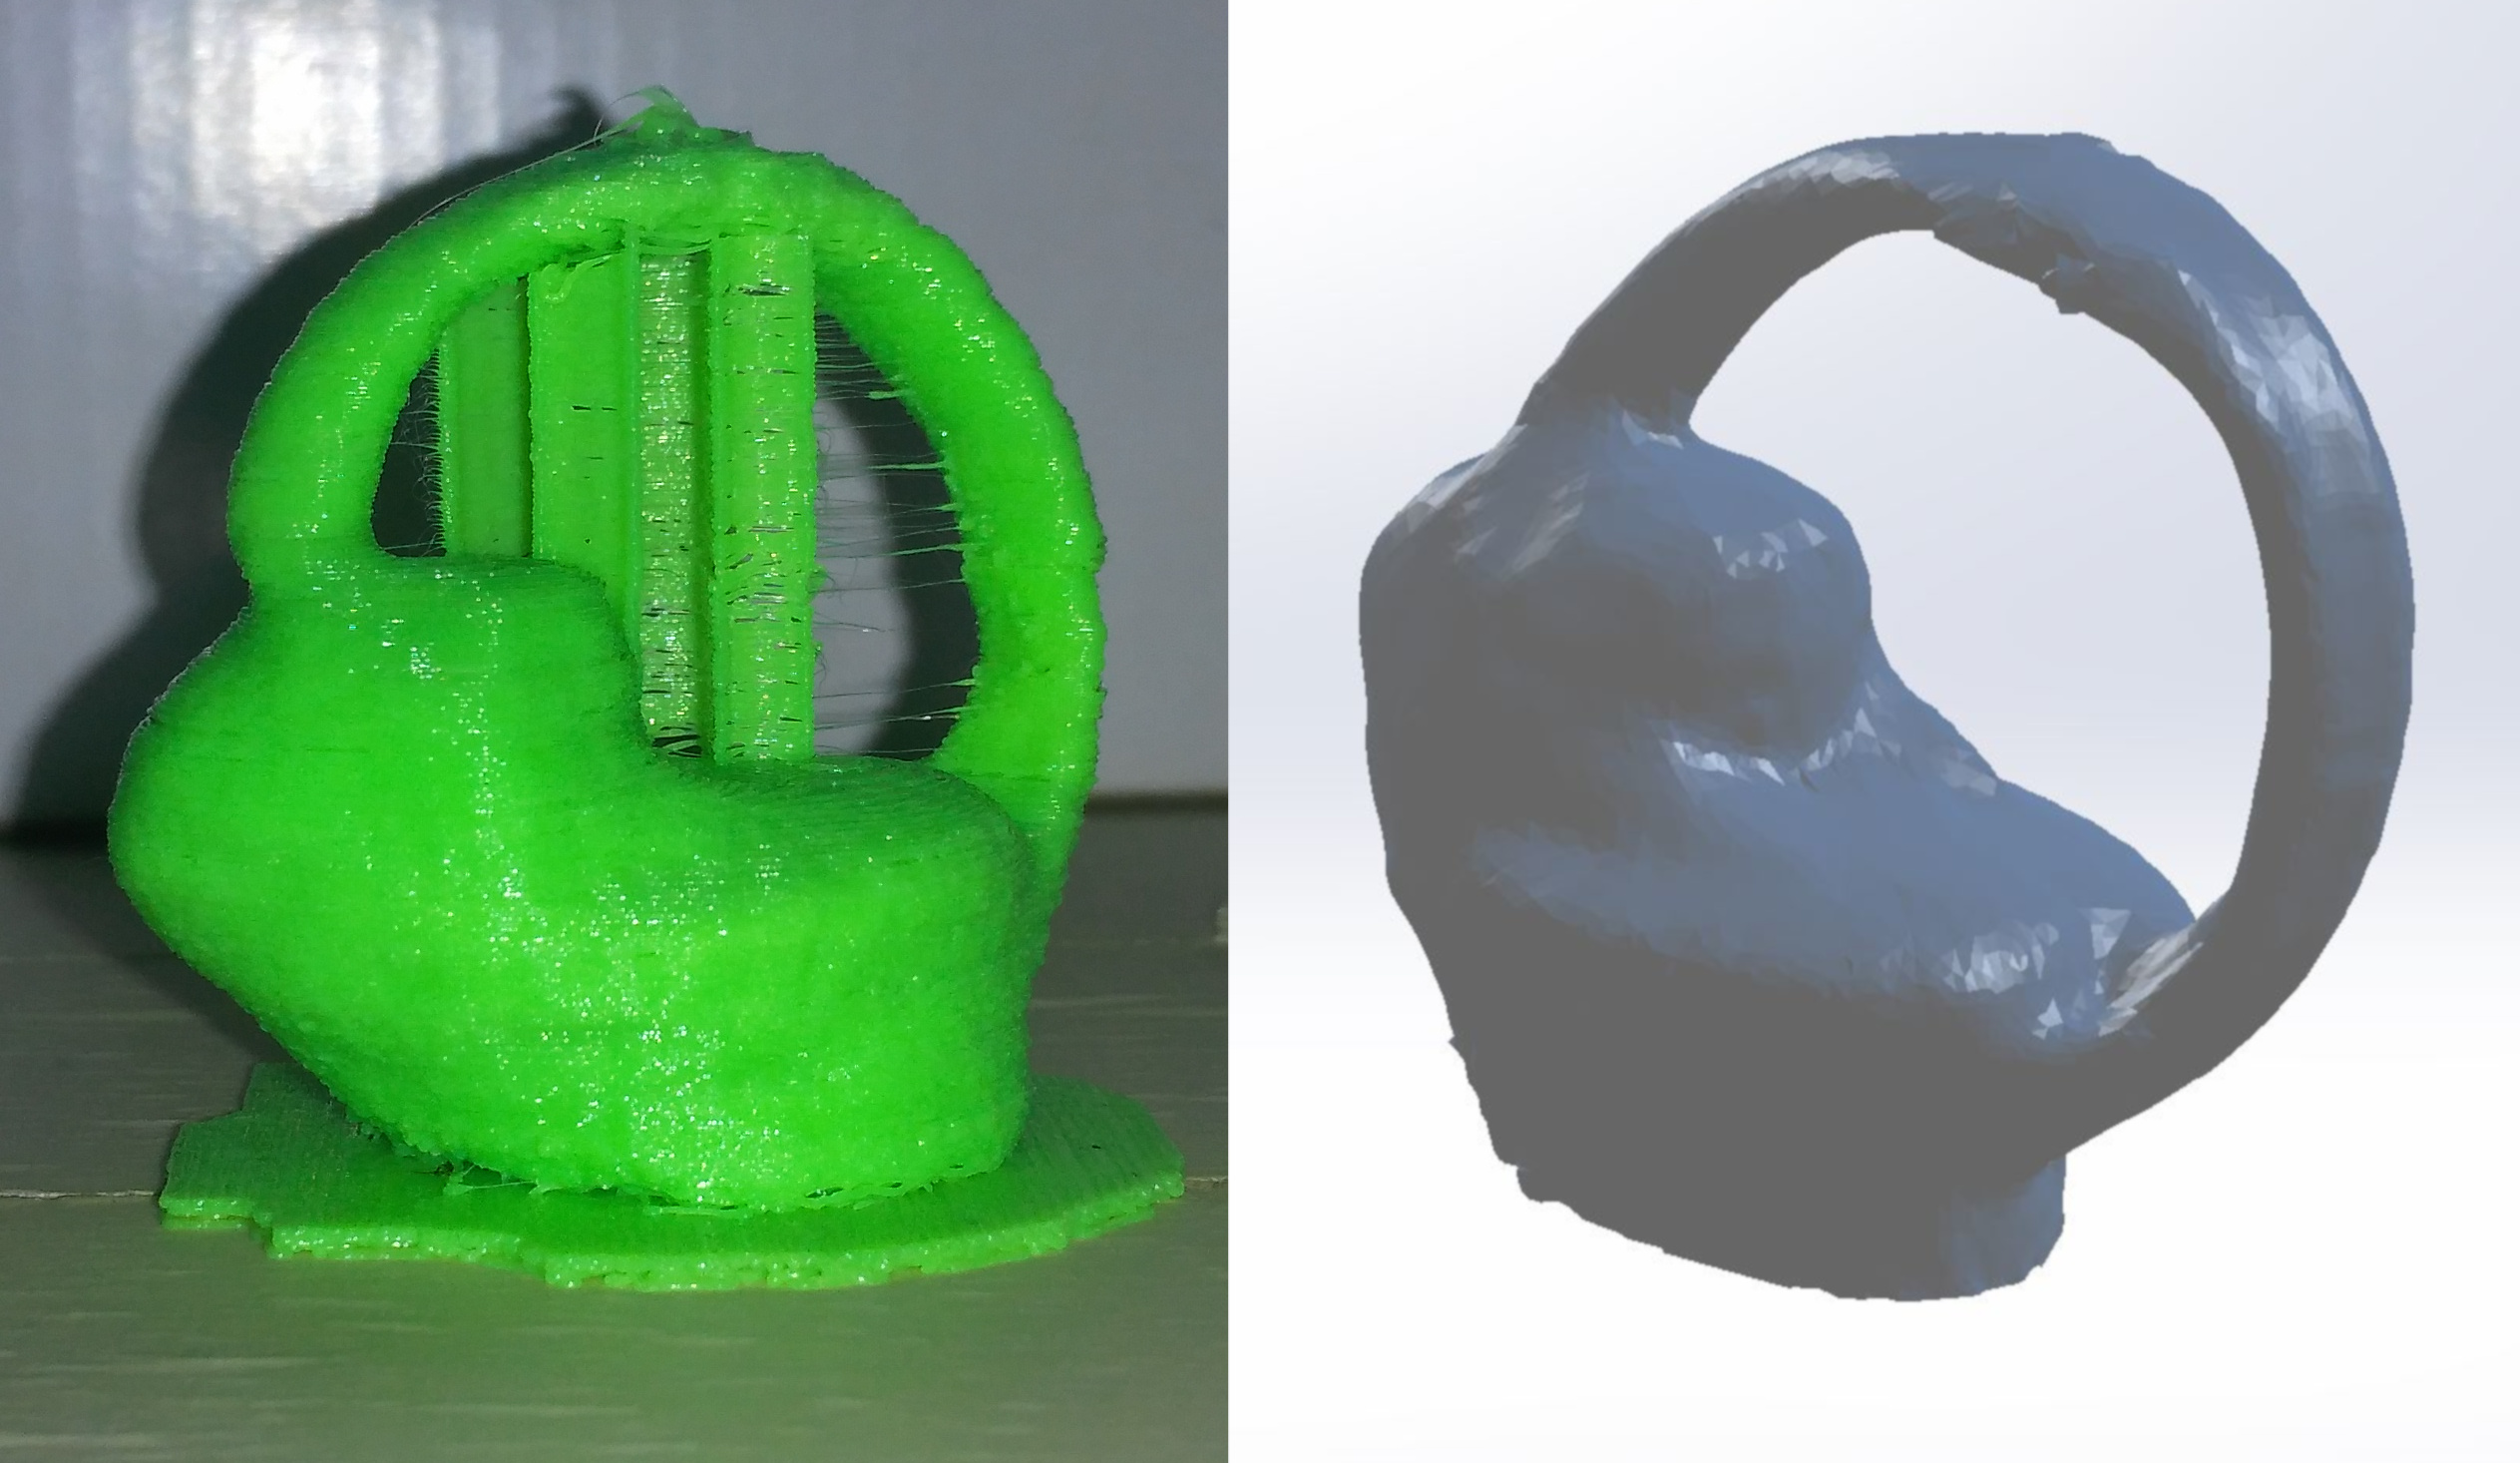
\includegraphics[width=8cm]{fig/print_slusalke}}
	\caption{Model po tiskanju ter lupina modela v modelirniku.}
	\label{fig:print_slusalke}
\end{figure}


\section{Zaključek}
Tekom izvajanja naloge smo ugotovili, da postopek 3D FBP rekonstrukcije dobro deluje pri popisu predmetov brez majhnih detajlov. Če pogledamo sliko \ref{fig:slika_90_30} vidimo, da rekonstruiran oblak točk modela ožilja ne vsebuje manjših žilic. Na kvaliteto rekonstrukcije močno vplivamo s številom zajetih slik ter z ustrezno osvetlitvijo, tako se znebimo črtastih arftefaktov, ki nastanejo s postopkom FBP. Pri tem pa je potrebno omeniti, da se čas rekonstrukcije močno poveča z večjim številom slik. Z pojmom dobra osvetlitev pa mislimo velik kontrast med ozadejm ter slikanim predemtom. Uporabljen algoritem rekonstrukcije omogoča tudi dimenzijsko analizo.

Poravnava oblakov se je izkazala za izredno uspešno kot to prikazuje tudi graf na sliki \ref{fig:poravnava_graf}. Pri pretvorbi digitalnega modela v fizičnega pa smo ugotovili, da na kvaliteto rezultirajočega modela močno vpliva vrsta algortima za izluščevanje točk površine, transformacija oblaka točk v 3D model ter sam postopek 3D tiskanja.

%Z našo tehniko rekonstruiranja nismo popisali dovolj dobrih delailov, čas rekonstrukcije se povečjuje z velikostjo sempljanja, ugotovili smo, da je sistem zelo pomemben + osvetlitev. Pomembno tud število slik. Poravnava slik, nam je dobro uspela - lahko če ne bi poznali pod kakšnim kotom je poslikal in dobil koliko je zamaknjen glede na referenčno lego.


\begin{thebibliography}{10}
\bibitem{spic1} Ž. Špiclin, B. Likar, M. Burmen. {\em Predavanje pri predmetu - Biomedicinske slikovne tehnologije: Rekonstrukcija slik}, \hskip 1em plus 0.5em minus 0.4em \relax Univerza v Ljubljani, 2018.
\bibitem{spic2} Ž. Špiclin. {\em Predavanje pri predmetu - Robotski vid: Prileganje modelov na slike}, \hskip 1em plus 0.5em minus 0.4em \relax Univerza v Ljubljani, 2019.
\bibitem{vir1} Moons, Theo, Luc Van Gool.  {\em 3D reconstruction from multiple images part 1: Principles}, \hskip 1em plus 0.5em minus 0.4em \relax Foundations and Trends in Computer Graphics and Vision 4.4: 287-404, 2010.
\bibitem{vir2}Vosselman, George, and Sander Dijkman.   {\em 3D building model reconstruction from point clouds and ground plans}, \hskip 1em plus 0.5em minus 0.4em \relax International archives of photogrammetry remote sensing and spatial information sciences 34.3/W4: 37-44, 2001.
\bibitem{vir3} Woodham, Robert J.  {\em  Photometric method for determining surface orientation from multiple images}, \hskip 1em plus 0.5em minus 0.4em \relax Optical Engineering. 19 (1): 138–141, 1980.
\bibitem{vir4}   {\em Raspberry Pi 3, Model B V1.2 Technical Specifications}, \hskip 1em plus 0.5em minus 0.4em \relax RS Components, 20.9.2017.
\bibitem{}   {\em Fischertechnik Technical Specifications}, \hskip 1em plus 0.5em minus 0.4em \relax fischertechnik GmbH, 2016.

\bibitem{}   {\em }, \hskip 1em plus 0.5em minus 0.4em \relax , 
\bibitem{}   {\em }, \hskip 1em plus 0.5em minus 0.4em \relax , 



\end{thebibliography}



\vfill

\label{finish}

% that's all folks
\end{document}


